\documentclass{article}[11pt]
\usepackage[utf8]{inputenc}
\usepackage{graphicx}
\usepackage{hyperref}
\usepackage{fancyhdr}
\usepackage{comment}
\usepackage{subcaption}
\usepackage{float}
\usepackage{geometry}
\usepackage{wrapfig}
\usepackage{multirow}

\usepackage[inline]{enumitem}
\hypersetup{ % color of index
    colorlinks,
    citecolor=black,
    filecolor=black,
    linkcolor=black,
    urlcolor=black
}
%\newgeometry{hmargin={30mm,40mm}}
\title{\vspace{-2.0cm}Computational Intelligence: FUZZY SYSTEMS
                        }
\author{Joan Llop Palao - Jordi Armengol Estapé}
\date{}

\begin{document}

\maketitle

\subsubsection*{1. Description of the membership functions for the output and rules}

\paragraph{Membership functions } \textbf{Implemented in} \texttt{pendulum\_controlle.fis} and \texttt{compound\_pendulum.slx}. Given a compound pendulum, the error of the angle and the derivative of the error, we want to develop a fuzzy system that controls the thrust of the propeller. The membership functions for the output variable correspond to the thrust being \textit{Positive} (ie. counterclockwise thrust), \textit{Neutral} (ie. no thrust) and \textit{Negative} (ie. clockwise thrust). There are multiple options regarding the shape of the membership functions (triangular, gaussian, ...). We could not find any differences between the surfaces generated by Gaussian membership functions and triangular membership functions. Thus, we use the latter since they are the default option. We considered different options with regard to the triangles form, but the option represented in figure \ref{fig:output_function_1} generated a very smooth surface (combined with most of the defuzzification functions). To choose a defuzzification function we plotted them in figure \ref{fig:defuzzification} and observed that centroids matched the idea on how our function should be.
\begin{figure}[htb!]
    \centering
    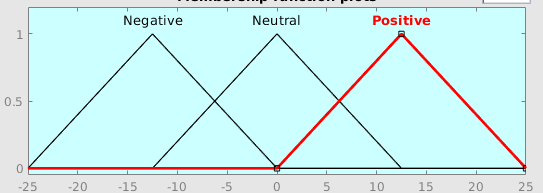
\includegraphics[width=0.5\textwidth]{img/output_variable_trinf_extended.png}
    \caption{Output membership functions}
    \label{fig:output_function_1}
%    \newline
%\end{figure}
%\begin{figure}[hbt!]
    \centering
    \centerline{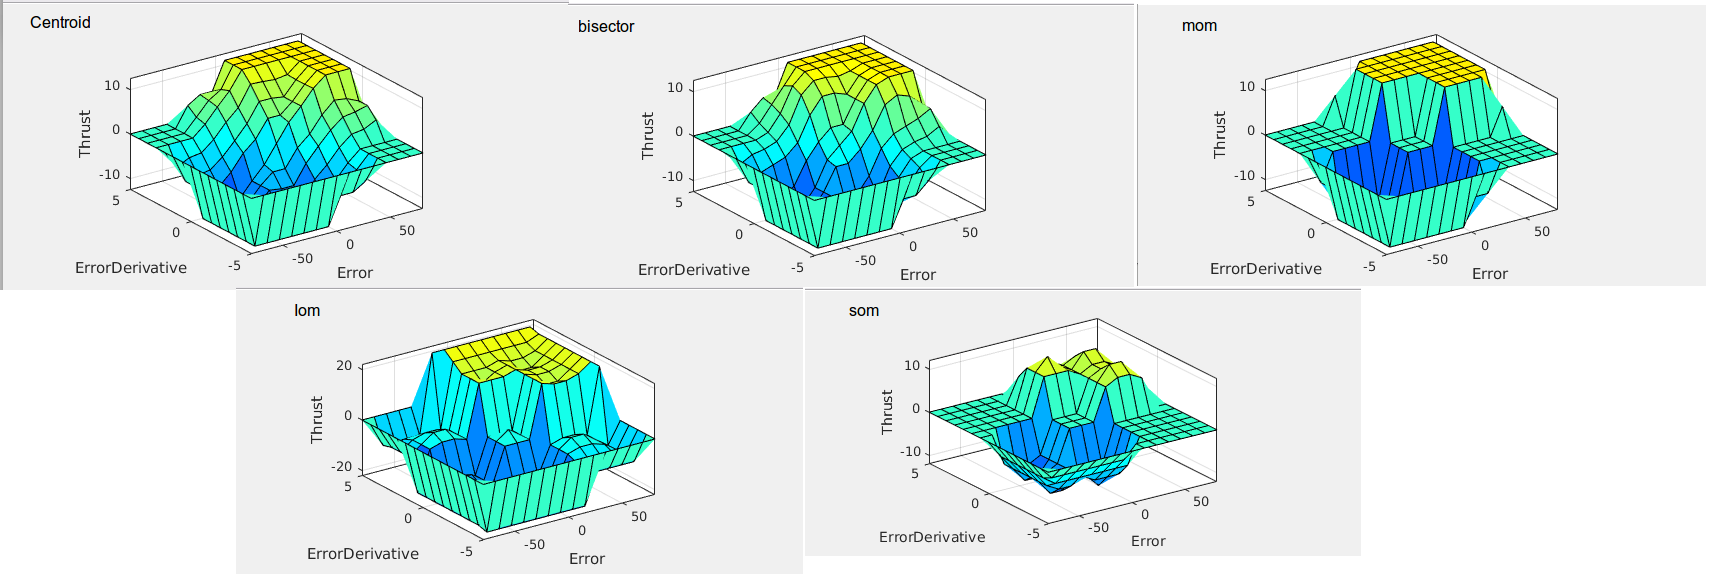
\includegraphics[width=\textwidth]{img/defuzzification.png}}
    \caption{Different surfaces with different defuzzification functions}
    \label{fig:defuzzification}
\end{figure}

\paragraph{Rules} The rules that are implemented in \texttt{pendulum\_controller.fis}. To justify them, we identify three cases:
\begin{enumerate*}
    \item \textbf{The error is worsening} (negative error and negative derivative, positive error and positive derivative, or zero error and positive or negative derivative): We have to change the direction (the thrust will be positive when the error is positive or when the error is zero and the derivative is positive and negative when the error is negative or zero and the derivative is negative).
     \item \textbf{The error is static (zero derivative)}: If the error is positive or negative we have to decrease it in the same way as when the error is worsening. When the error is zero we do nothing because we already have the ideal angle.
     \item \textbf{The error is getting better}: We do nothing because we are getting closer to the ideal angle. We have considered to push the pendulum in order to keep improving the error in a quicker manner, but we discarded the option because we could cause oscillations when the ideal angle is close to the real one.
\end{enumerate*} From this reasoning, we derive the \textbf{9} rules:

\begin{center}
\hspace*{-1.3cm}\begin{tabular}{|c|l|c|c|}
    \hline
    \multirow{2}{*}{\bfseries Rule} & 
    \multicolumn{2}{|c|}{\bfseries Condition} & \multirow{2}{*}{\bfseries Thrust} \\ \cline{2-3} & Error & Deriv& \\ \hline
    %------
    1 & Neg & Decr & Neg\\
    2 & Neg & Stat & Neg\\
    3 & Neg & Incr & Neu\\
    \hline
\end{tabular}
\hfill
\begin{tabular}{|c|l|c|c|}
    \hline
    \multirow{2}{*}{\bfseries Rule} & 
    \multicolumn{2}{|c|}{\bfseries Condition} & \multirow{2}{*}{\bfseries Thrust} \\ \cline{2-3} & Error & Deriv& \\ \hline
    %------
    4 & Zer & Decr & Neg\\
    5 & Zer & Stat & Neu\\
    6 & Zer & Incr & Pos\\
    \hline
\end{tabular}
\hfill
\begin{tabular}{|c|l|c|c|}
    \hline
    \multirow{2}{*}{\bfseries Rule} & 
    \multicolumn{2}{|c|}{\bfseries Condition} & \multirow{2}{*}{\bfseries Thrust} \\ \cline{2-3} & Error & Deriv& \\ \hline
    %------
    7 & Pos & Decr & Neu\\
    8 & Pos & Stat & Pos\\
    9 & Pos & Incr & Pos\\
    \hline
\end{tabular}
\end{center}

\begin{comment}


\begin{enumerate}
    \item if (Error is Negative) and (ErrorDerivative is Decreasing) then (Thrust is Negative).
    \item if (Error is Negative) and (ErrorDerivative is Stationary) then (Thrust is Negative).
    \item if (Error is Negative) and (ErrorDerivative is Increasing) then (Thrust is Neutral).
    \item if (Error is Zero) and (ErrorDerivative is Decreasing) then (Thrust is Negative).
    \item if (Error is Zero) and (ErrorDerivative is Stationary) then (Thrust is Neutral).
    \item if (Error is Zero) and (ErrorDerivative is Increasing) then (Thrust is Positive).
    \item if (Error is Positive) and (ErrorDerivative is Decreasing) then (Thrust is Neutral).
    \item if (Error is Positive) and (ErrorDerivative is Stationary) then (Thrust is Positive).
    \item if (Error is Positive) and (ErrorDerivative is Increasing) then (Thrust is Positive).
\end{enumerate}
\end{comment}

\begin{comment}
\begin{itemize}
    \item \textbf{The error is increasing} (negative error and negative derivative, or, positive error and positive derivative, or zero error and positive or negative derivative) we have to stop increasing the error and start decreasing it (The Thrust will be positive when the error is positive or when the error is zero and the derivative is positive and negative when the error is negative or zero and the derivative is negative).
     \item \textbf{The error is static (zero derivative)} if the error is positive or negative we have to decrease it in the same way as when the error is increasing, when the error is zero we do nothing because we already have the ideal angle.
     \item \textbf{The error is decreasing} we do nothing because we are getting closer to the ideal angle. We have considered to push the pendulum in order to keep decreasing the error in a quicker manner, but we discarded the option because we could provoke oscillations when the ideal angle is close to the real one.
\end{itemize}
\end{comment}
\subsubsection*{2. Plot of the results with a simulation stop time of 80}
As we can observe in the plots \ref{fig:sub1} and \ref{fig:sub2}, the rules we have defined have successfully stopped the pendulum from oscillating. In both cases (positive and negative ideal angle) our fuzzy controller has shown a neat approximation to the ideal angle and a quicker stabilization than the original.% system. %Thus, we expect it to work with any desired angle.
\begin{figure}[H]
\centering
\hspace*{-1cm}\begin{subfigure}{.6\textwidth}
  %\centering
  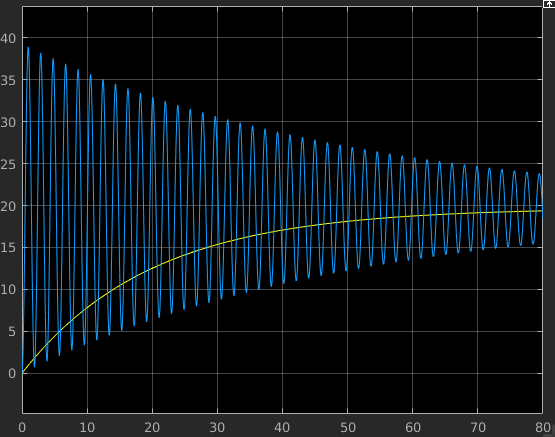
\includegraphics[width=0.9\linewidth]{img/result_20_2.png}
  \caption{Output with $theta\_ref = 20$ and $thrust = 0.123$}
  \label{fig:sub1}
\end{subfigure}%
\hspace*{-1cm}\begin{subfigure}{.6\textwidth}
  \centering
  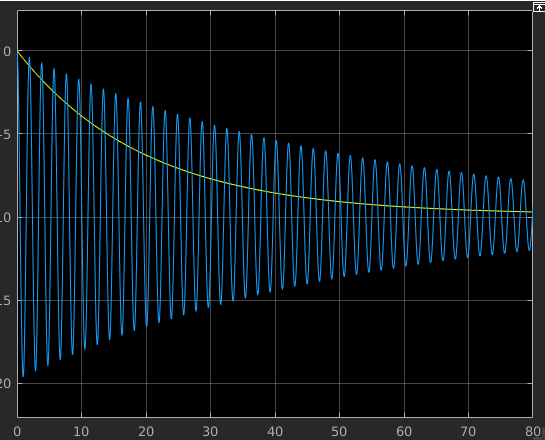
\includegraphics[width=0.9\linewidth]{img/result_minus10.png}
  \caption{Output with $theta\_ref = -10$ and $thrust = -0.062$}
  \label{fig:sub2}
\end{subfigure}
\caption{The pendulum oscillation (blue) and the pendulum stabilized with our system (yellow)}
\label{fig:test}
\end{figure}
\begin{comment}
\begin{itemize}
    \item \textbf{$theta\_ref = 20$ and $thrust = 0.123$} can be found in image \ref{fig:results_20}
        \begin{figure}[hbt!]
            \centering
            \centerline{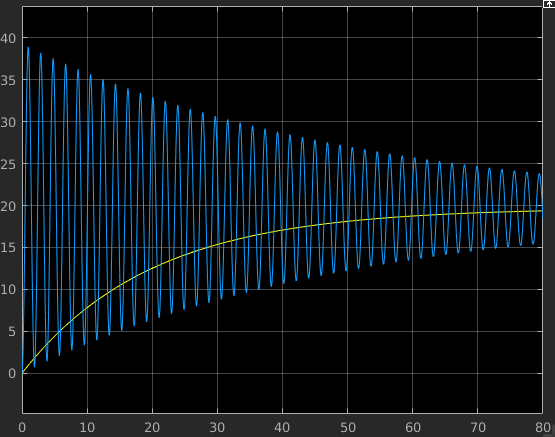
\includegraphics[]{img/result_20_2.png}}
            \caption{Output with $theta\_ref = 20$ and $thrust = 0.123$}
            \label{fig:results_20}
        \end{figure}
        
    \item \textbf{$theta\_ref = -10$ and $thrust = 0.062$} can be found in image \ref{fig:results_-10}
        \begin{figure}[hbt!]
            \centering
            \centerline{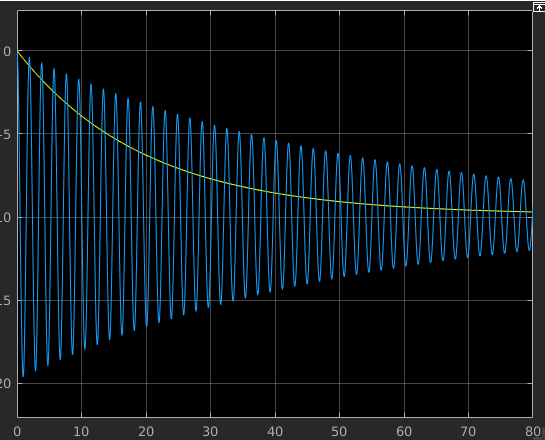
\includegraphics[]{img/result_minus10.png}}
            \caption{Output with $theta\_ref = -10$ and $thrust = -0.062$}
            \label{fig:results_-10}
        \end{figure}
\end{itemize}
As we can observe in the plots (\ref{fig:results_20}, \ref{fig:results_-10}) the set of rules that we have defined have successfully stop the pendulum from oscillating. In both cases (positive and negative ideal angle) our fuzzy controller has shown a very neat approximation to the ideal angle, therefore we expect it to work with any desired angle. 
\end{comment}
\subsubsection*{3. What happens if we increase the number of membership functions of the output? }
\textbf{Implemented in} \texttt{pendulum\_controller\_5\_output.fis}. If we increase the number of mfs, the resulting surface is smoother, since we specify more fine-grained rules for the problem (eg. soft thrust if the error is non-zero but at least it is not getting worse). We have implemented an output function with 5 triangular mfs: very\_negative, negative, neutral, positive and very\_positive. The observed results are similar to the ones obtained with 3 mfs (see attached image in \texttt{img/result\_5\_outputs.png})

\end{document}
